\documentclass[12pt, letterpaper]{article}
\title{Actividad 3}
\author{}
\date{Semana 2}
\usepackage[style=apa,sortcites=true,sorting=nyt,backend=biber]{biblatex}
\DeclareLanguageMapping{spanish}{spanish-apa}
\usepackage{listings}
\usepackage{xcolor}
\usepackage{graphicx}


% Define a custom color
\definecolor{backcolour}{rgb}{0.95,0.95,0.92}
\definecolor{codegreen}{rgb}{0,0.6,0}

% Define a custom style
\lstdefinestyle{myStyle}{
    backgroundcolor=\color{backcolour},   
    commentstyle=\color{codegreen},
    basicstyle=\ttfamily\footnotesize,
    breakatwhitespace=false,         
    breaklines=true,                 
    keepspaces=true,                 
    numbers=left,       
    numbersep=5pt,                  
    showspaces=false,                
    showstringspaces=false,
    showtabs=false,                  
    tabsize=2,
}
\lstset{style=mystyle}

 \addbibresource{demo.bib}
\begin{document}
\begin{titlepage}
\centering
{\bfseries\LARGE Universidad del Valle de México \par}
\vspace{1cm}
{\scshape\Large Laureate International Universities  \par}
\vspace{3cm}
{\scshape\Huge Estadística Descriptiva e Inferencial  \par}
\vspace{2cm}
{\itshape\Large Actividad 3  \par}
\vfill
{\small Autor: \par}
{\Large Vladimir Armando Salgado Loezza \par}
\vspace{1cm}
{\small Matricula: \par}
{\Large 940029771\par}
\vspace{1cm}
{\small Profesor: \par}
{\small Mtro. Marco Antonio Hernández De Ita\par}
\vspace{1cm}
{\small Noviembre 2023 \par}
\end{titlepage}
 




 
\maketitle


La empresa, “La casa de la abue”, se dedica desde hace más de 5 años a la
elaboración de repostería fina. Está ubicada en la ciudad de México, en la zona
Sur. Desde hace poco más de medio año, inició con la incursión de un nuevo
producto en su cartera: los cupcakes.
Debido a que se tiene poca experiencia en éste nuevo producto, no se ha logrado
encontrar un estándar en cuanto al producto final. Los pasteles que ofrece y la
pasta seca, se caracterizan, además del sabor, por su estandarización tanto en
la presentación, cómo en los ingredientes.
En el último lote que se elaboró, se pesaron cada uno de los cupcakes que se
hicieron. La siguiente lista representa el peso en gramos de cada uno de los
pastelitos:
\begin{center}
 
50.3, 50.5, 50.8, 51.3, 51.7, 51.3, 51.1, 51.4, 51.3, 51.6, 50.2, 50.5,
50.7,50.0, 51.1, 50.4 ,50.6, 51.2, 50.4, 50.8, 50.2 , 50.6, 51.2, 50.4,
50.8, 50.2, 50.6, 49.4, 49.6, 50.8, 49.9 , 50.4, 50.1, 51.0, 49.3, 49.5,
49.1, 50.9 , 49.6, 49.8, 49.5, 49.7, 50.0, 51.1, 49.7, 50.3, 50.4, 50.8, 49.9,
51.7, 50.0, 50.2, 49.2, 49.1, 49.2, 51.1, 50.8, 49.7, 50.5, 50.4, 49.5, 49.7,
50.5, 50.3, 50.0, 50.1, 49.1, 51.4, 50.9, 49.1, 50.6, 50.4, 50.6, 49.7,
49.2, 50.1, 49.9, 49.6, 50.7, 49.3, 50.2, 50.7, 49.3, 49.3, 50.3, 49.1, 49.9,
49.8, 50.3, 50.1, 50.5, 49.5, 50.8, 50.0, 50.7, 50.5, 49.4, 50.7, 49.1,
50.8, 50.6, 49.1, 49.3

\end{center}
    \newpage



\textbf{  Etapa 1.}
\begin{enumerate} 
    \item Obtener la estadística descriptiva según los datos proporcionados.

\begin{enumerate}
    \item \textbf{Moda:} 50.8
    \item \textbf{Media:} 50.23883495145631
    \item \textbf{Mediana:} 50.3
    \item \textbf{Varianza:} 0.4625695164482992
    \item \textbf{Desviación estándar:} 0.6801246330256677
    
\end{enumerate}    
Los datos se obtuvieron con el siguiente código en Python, así mismo se usó matplotlib para la gráfica, el código  se encuentra en el archivo “main.py”, 
 este código se obtuvo mediante el análisis de la estadística descriptiva del libro de texto \cite{Probabilidad} en las páginas 40,41,44.:
\begin{lstlisting}[language=Python]
        import flet as ft
        import math
        import statistics
        import matplotlib
        import matplotlib.pyplot as plt
        from flet.matplotlib_chart import MatplotlibChart

        ....

 
            
            c1 = ft.Column()
            
            pesos = [50.3, 50.5, 50.8, 51.3, 51.7, 51.3, 51.1, 51.4, 51.3, 51.6, 50.2, 50.5, 50.7, 50.0, 51.1, 50.4, 50.6, 51.2, 50.4, 50.8, 50.2, 50.6, 51.2, 50.4, 50.8, 50.2, 50.6, 49.4, 49.6, 50.8, 49.9, 50.4, 50.1, 51.0, 49.3, 49.5, 49.1, 50.9, 49.6, 49.8, 49.5, 49.7, 50.0, 51.1, 49.7, 50.3, 50.4, 50.8, 49.9, 51.7, 50.0, 50.2, 49.2, 49.1, 49.2, 51.1, 50.8, 49.7, 50.5, 50.4, 49.5, 49.7, 50.5, 50.3, 50.0, 50.1, 49.1, 51.4, 50.9, 49.1, 50.6, 50.4, 50.6, 49.7, 49.2, 50.1, 49.9, 49.6, 50.7, 49.3, 50.2, 50.7, 49.3, 49.3, 50.3, 49.1, 49.9, 49.8, 50.3, 50.1, 50.5, 49.5, 50.8, 50.0, 50.7, 50.5, 49.4, 50.7, 49.1, 50.8, 50.6, 49.1, 49.3]
            
            data_input=ft.TextField(label=str(pesos))
            
            # Calcula la suma de los elementos del grupo de datos
            suma = sum(pesos)

            #Numero de n elementos en el grupo de datos
            longitud = len(pesos)
            
            # Calcula la media aritmetica del grupo de datos
            media = suma/longitud

            # Calcula la moda
            moda = statistics.mode(pesos)
            #calcula la mediana
            mediana = statistics.median(pesos)

            # Calcula la suma de los cuadrados de las diferencias
            suma_cuadrados_diferencias = sum((x - media) ** 2 for x in pesos)

            # Calcula la varianza
            varianza = suma_cuadrados_diferencias / len(pesos)

            # Calcula la desviacion estandar
            desviacion_estandar = math.sqrt(varianza)

           


            
\end{lstlisting}

    
\item Del archivo “Información Proyecto Integrador.docx”, captura en Excel los datos de los pesos de los cupcakes. 
    Para esto se te solicita que obtengas dos columnas, la primera con el número de cupcakes que se está analizando 
    y en la segunda columna el peso en gramos del mismo. 
    Coloca nombre a cada una de las columnas y dale un formato adecuado. Cambia el nombre de la hoja por “Datos”.

   \begin{center}%
   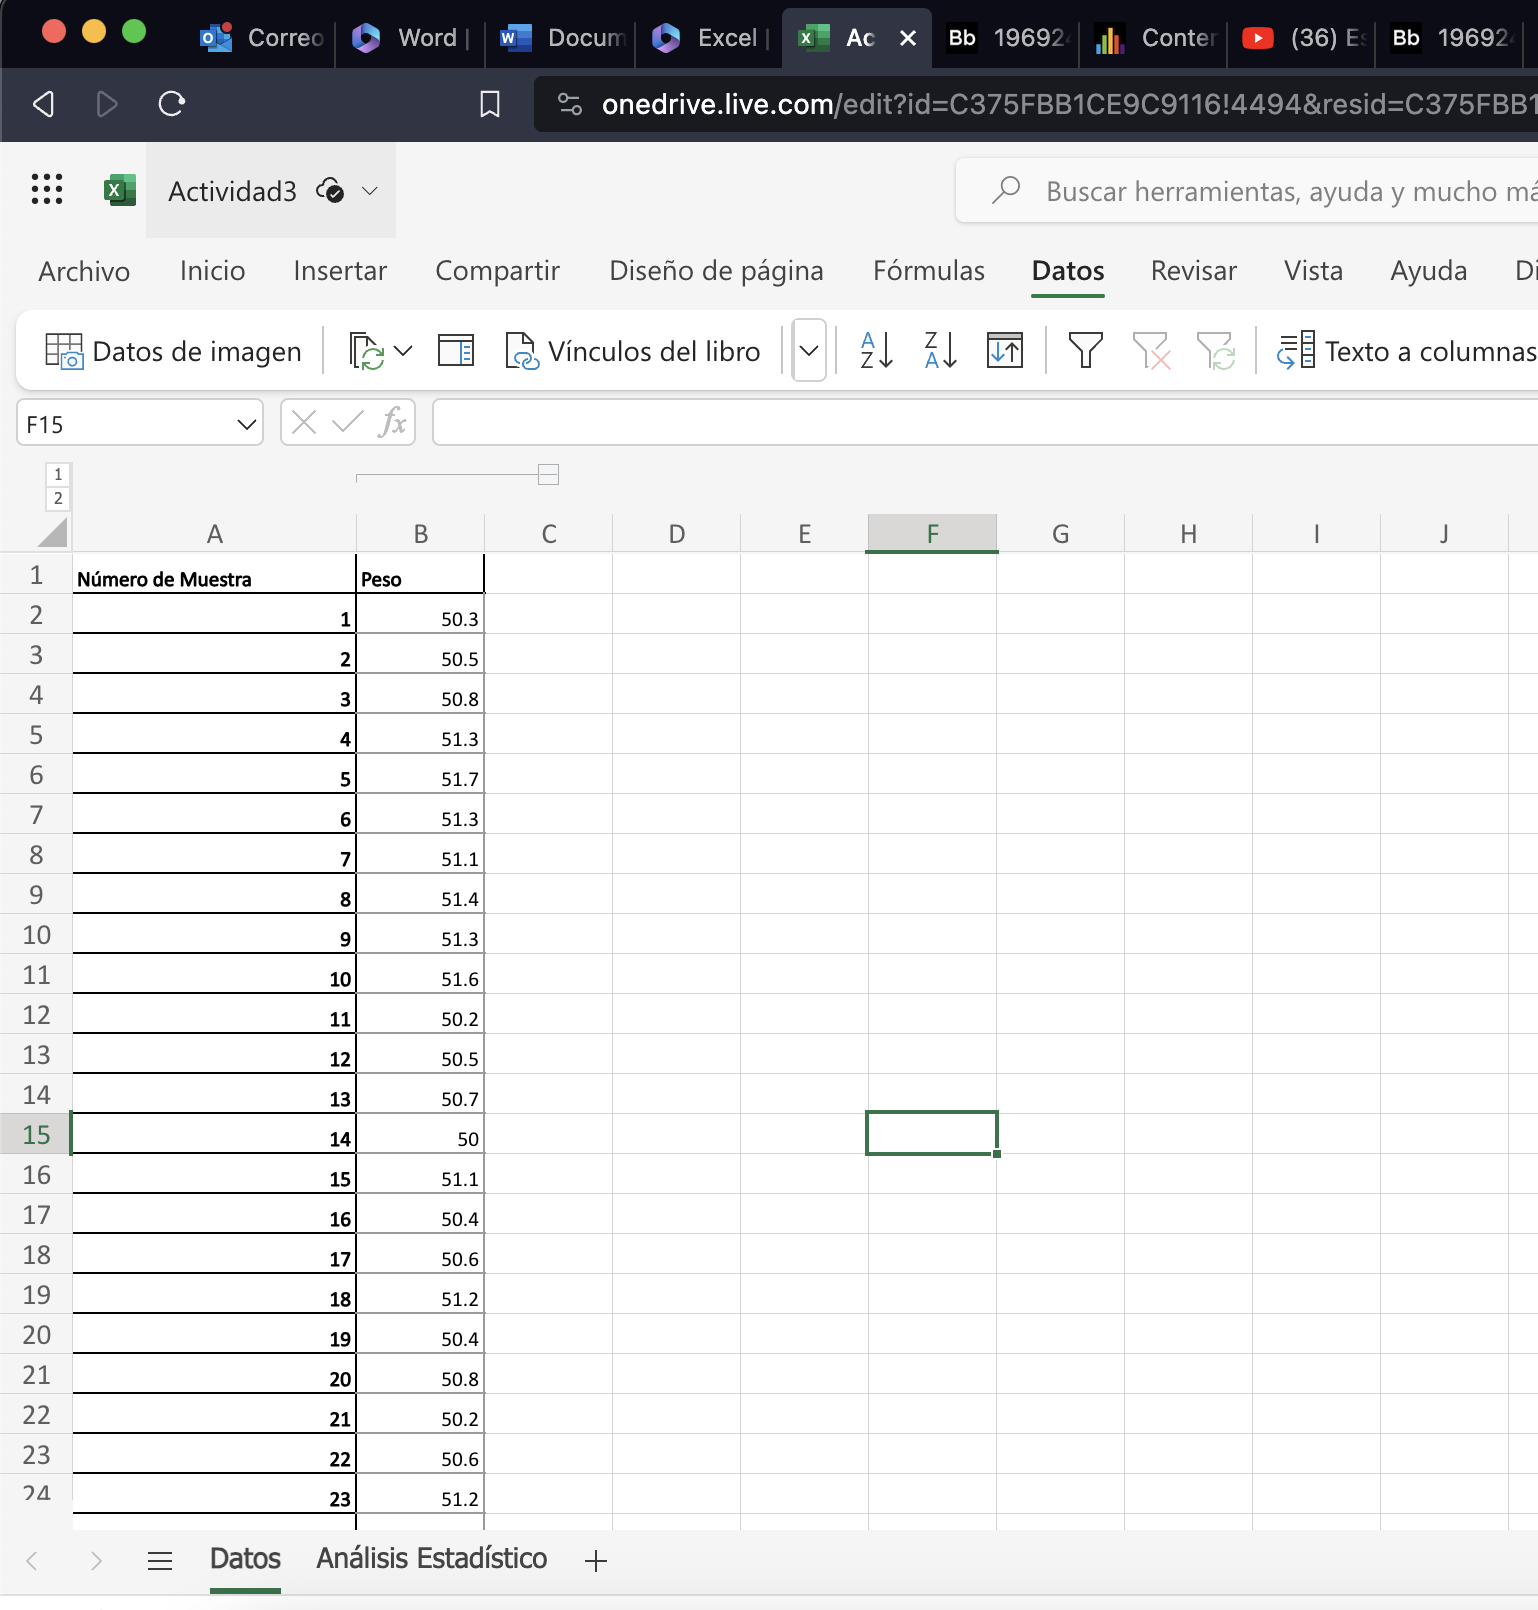
\includegraphics[width=300pt]{act3_evidencia2.png}
    \end{center}
 
\end{enumerate}

 \begin{thebibliography}{Referencias}
    \bibitem{Baz} \textsc{William Mendellhall,} y \textsc{Terry Sincich},
    \textit{Probabilidad y estadística para ingeniería Y Ciencias}, cuarta edición,
    Prentice Hall, México, DF, 2017.  \textbf{ págs. 2, 40,41,44.}
\end{thebibliography}
   
  
\end{document}